\summary
Representation learning lives at the heart of deep learning for natural language processing (NLP). 
Traditional representation learning (such as softmax-based classification, pre-trained word embeddings, and language models, graph representations) focuses on learning general or static representations with the hope to help any end task.
As the world keeps evolving, emerging knowledge (such as new tasks, domains, entities or relations) typically come with a small amount of data with shifted distributions that challenge the existing representations to be effective.
As a result, how to effectively learn representations for new knowledge becomes crucial.
Lifelong learning is a machine learning paradigm that aims to build an AI agent that keeps learning from the evolving world, like humans' learning from the world.
This dissertation focuses on improving representations on different types of new knowledge (classification, word-level, contextual-level, and knowledge graph) for a myriad of NLP end tasks, ranging from text classification, sentiment analysis, entity recognition, question answering to the more complex dialog system.
With the help of lifelong representation learning, models' performance on tasks is greatly improved beyond existing general representation learning.

\chapter{Introduction}
\label{chap1:intro}

Deep learning (DL) has achieved significant performance boosts for machine learning tasks over the past a few years\cite{Goodfellow-et-al-2016-Book}. 
The core driving force behind deep learning is its capability or capacity to learn knowledgable features or representations automatically from large-scale data.
This significantly reduces the need for asking humans to curate better features manually.
As a result, the learned representation gives the model a great advantage to concur with the uncertainty during testing from the unknown world, which can be found in many applications of computer vision and natural language processing.
The key advantage of deep learning over traditional machine learning models is that by having parameter-intensive models, deep learning models can consume much more data to obtain more general representation by inferring the features on-the-fly as a form of stacked layers of reasoning. 
Thus, those features shorten the gap between the raw inputs and the features required by an end task.
Not surprisingly, these learned features, in the end, boost the performance of many tasks.

Following this advantage, how to smartly consume more data to learn general features and avoid specific features is essential for the success of DL models.
Researchers start to pre-train DL models with the hope to encode all features of the world into parameters of DL models.
Examples can be found in the large-scale pre-training on ImageNet dataset \cite{deng2009imagenet,russakovsky2015imagenet,krizhevsky2012imagenet} in computer vision, or pre-trained word embeddings or language models \cite{peters2018deep,devlin2018bert} in natural language processing (NLP).

\section{Motivation of Lifelong Learning}
\label{chap1:motivation}
Going beyond the classic deep learning approach, simply aggregating existing data into a DL model may not be enough.
For example, looking towards the future, the world keeps evolving and always yields new data for new tasks, which probably are long-tailed or heavily-tailed.
This greatly challenges the existing learned representations.
This is because a trained model is typically frozen during inference or testing and never changed.
The existing approach may represent the majority general features well and assume they are generally good for any new knowledge.
However, it lacks enough capability to represent the vast kinds of specific features that are required each (new) task.
To make the learning effective in the long-term, an AI agent must be able to adapt to the changes in the world.
In contrast, we humans are very sensitive to the changes in the world and the wide spectrum of novel details by having a focus with curiosity on new things.
Later we learn new knowledge and updating our understanding of the world.
In contrast to the existing machine learning paradigm, we never use our 6-year-old understanding of the world to solve the problems now. 

\section{Research Objectives}
Motivated by this observation, an AI agent needs to learn representations as to the way humans do in a new machine learning paradigm or a problem called \textbf{lifelong learning}, which aims to build AI agents from a sequence of tasks online.

\textit{Lifelong Learning} (LL) assumes that the learning tasks come in a sequence denoted as $\mathcal{T}_1, \mathcal{T}_2, \dots, \mathcal{T}_n$, where the new or $(n+1)$-th task is performed with the help of the knowledge accumulated over the past $n$ tasks \cite{thrun1998lifelong,silver2013lifelong,chen2018lifelong}. 

Note that this definition does not specify or constrain the forms or types of each task.
To name a few, a task can be any learning task, ranging from learning for a new class, learning for a new domain, learning in a heterogeneous form of a new task, to new concept or relation for accumulating the knowledge.
As such, we can see that the problem or concept of lifelong learning can be applied to a vast amount of concrete machine learning tasks.

As a result, this dissertation focuses on a wide range of machine learning tasks and their usage in natural language processing (NLP) applications.
We aim to cover major types of machine learning tasks in NLP and provide its applications to concrete datasets with experimental results and discussions on the role of lifelong learning for the improvements in their models' performance.

\section{Outlines}
To make a more clear distinction between different forms of learning tasks and NLP applications, this dissertation is organized by separating lifelong learning tasks of different types and their applications to concrete NLP tasks. As a result, the structure of this dissertation may not exactly follow the structure of the papers published in their original form. To build the relevance with the original paper, I list referenced papers at the beginning of each chapter. 

In Chapter \ref{chap2:open}, I first address open-world learning problems on classification tasks, where traditional classifiers can easily make mistakes on unseen classes that appear during testing or inference. 
This is because most existing classifiers must classify an example from an unseen class to one of existing pre-defined classes during training. 
I further extend this problem to a dynamic classification task, where some unseen classes can be added to or removed from the set of existing classes while still keeping rejecting the rest unseen classes. We use a meta-learning approach to address this problem into a very general comparison-based classifier.
As a result, it avoids learning a classifier overfitting to a particular set of classes.

In Chapter \ref{chap3:word}, I switch to classic representation learning problems in NLP.
I first focus on learning word embedding and propose a problem of learning domain word embeddings.
In this problem, each word has its domain representation.
However, emerging domains typically do not have enough corpus to train fully-fledged embeddings.
By applying lifelong learning into word embeddings, I allow corpus-level sharing of knowledge amongst existing domains. 
As such, I first describe how to obtain domain-specific word embeddings from a small domain corpus in a lifelong learning fashion and show the performance domain-specific embeddings compare to general-purpose embeddings.
Second, I explore the usage of domain-specific word embeddings and focus on how to leverage both general-purpose embeddings and domain-specific embeddings together.

In Chapter \ref{chap4:context}, I switch to contextualized word representation, where each word is strongly tied to its context in a document.
This yields a better representation of the meaning of a word in a sentence or paragraph.
Given the expensive training of contextualized word representation, I switch to a different style of lifelong learning and focuses on how to obtain domain contextualized word representation via a sequence of different types of learning tasks.
I discuss two types of learning tasks: post-training and pre-tuning.
On one hand, post-training is a learning task intended to address the shifts of distributions such as domains.
This ended with a huge gap between an end task and a general-purpose pre-trained contextualized word representation. 
Pre-tuning, on the other hand, aims to solve the discrepancy between a pre-trained contextualized word representation and end tasks.
Given existing pre-trained models aim to cover a wide range of end-tasks, the learned representation is not optimal for each end task.
The proposed pre-tuning task mimics the formulation of an end task with only unlabeled data, which shortens the gap between a pre-trained model and an end task.

Further, in Chapter \ref{chap5:graph}, I move towards graph representation learning.
A graph is a natural way for sharable and interpretable knowledge for humans.
It can be used for both feature augmentations and reasoning.
However, the existing approach of graph representation learning mostly assumes a static graph, where the knowledge and reasoning upon knowledge are never changed.
Lifelong learning is ideal for graph reasoning as it can keep updating graphs and reasoning policy.
Thus, we rename the term graph as a memory graph, indicating the graph is dynamic that can maintain and update reasoning based on newly added knowledge.

Lastly, in Chapter \ref{chap6:nlp}, I target the usage of lifelong learning over a wide spectrum of NLP tasks.
I first describe the tasks in aspect-based sentiment analysis (ABSA).
ABSA has two important subtasks: aspect extraction and aspect sentiment classification. 
I first describe the usage of domain word embeddings (from Chapter \ref{chap3:word}) and contextualized word representation (from Chapter \ref{chap4:context}) for aspect extraction.
Later I discuss the contextualized word representation and the lifelong training algorithm of hard examples for aspect sentiment classification.
One important issue associated aspect sentiment classification is lacking the capability to learn hard examples that are important for the aspect-level sentiment.
I address this problem by proposing a training algorithm that focusing on hard examples.
Next, I switch to a novel problem called complementary entity recognition (CER) in my early years of Ph.D. research.
I discuss two papers that have the capability of lifelong learning to accumulate past knowledge for entity extraction.
Then, I go through the question-answering problem and focus on machine reading comprehension (MRC) and its novel application to reviews.
Lastly, I discuss the usage of lifelong learning for conversational AI. 
I first describe the usage of pre-tuning for a novel problem called review conversational reading comprehension (RCRC).
Then focus on lifelong graph reasoning for conversational recommendation with dynamic graph reasoning (using the method in Chapter \ref{chap5:graph}).

\chapter{Lifelong Classification}
\label{chap2:open}

The content of this chapter was previously published as ``Open-world Learning and Application to Product Classification'' in WWW 2019 \cite{xu2019open}, DOI: https://doi.org/10.1145/3308558.3313644.
%, with an arXiv version \footnote{https://arxiv.org/abs/1809.06004} \cite{xu2018open}.

Classification is a well-known and classic problem and the deep learning variant of the classification task typically leverages an activation function that can compute a categorical distribution over a set of classes (e.g., the softmax function).
This type of classification is called \textit{closed-world classification} because the classes seen in testing must have appeared in training. However, this assumption is often violated in real-world applications. For example, new topics often emerge on a social media site and new categories of products appear daily on an e-commerce website. 
A model that cannot detect new/unseen topics or products is hard to function well in such open environments.  
This is where lifelong learning can be applied to the existing classification problem.

\section{Motivation}
Generally speaking, an AI agent working in the real world must be able to recognize the classes of things that it has seen/learned before and detect new types of things that it has not seen and later learn to accommodate the new things. This learning paradigm is called \textit{\underline{o}pen-\underline{w}orld \underline{l}earning} (OWL)
\cite{chen2018lifelong,bendale2015towards,fei2016learning}. 
This is in contrast with the well-known supervised learning paradigm, which makes the \textit{closed-world assumption}.
This assumption indicates that the classes in testing must have appeared during the stage of training. With the ever-changing Web, the popularity of AI agents such as intelligent assistants and self-driving cars that need to face the real-world open environment with unknowns, OWL capability is crucial.

For example, with the growing number of products sold on Amazon from various sellers, it is necessary to have an open-world model that can automatically classify a product based on a set $S$ of product categories.
An emerging product not belonging to any existing category in $S$ should be classified as ``unseen'' rather than one from $S$.
Further, this unseen set may keep growing. When the number of products belonging to a new category is large enough, it should be added to $S$.
An open-world model should easily accommodate this addition with a low cost of training since it is impractical to retrain the model from scratch every time a new class is added.
As another example, the very first interface for many \underline{i}ntelligent \underline{p}ersonal \underline{a}ssistants (IPA) (such as Amazon Alexa, Google Assistant, and Microsoft Cortana) is to classify user utterances into existing known domain/intent classes (e.g., Alexa's skills) and also 
reject/detect utterances from unknown domain/intent classes (that are currently not supported).
But, with the support to allow the 3rd-party to develop new skills (Apps), such IPAs must recognize new/unseen domain or intent classes and include them in the classification model. These real-life examples present a major challenge to the maintenance of the deployed model.

\section{Open-world Learning}
Most existing solutions to OWL are built on top of closed-world models \cite{bendale2015towards,bendale2016towards,fei2016learning,shu-xu-liu:2017:EMNLP2017}, e.g., by setting thresholds on the logits (before the softmax/sigmoid functions) to reject unseen classes which tend to mix with existing seen classes. One major weakness of these models is that they cannot easily add new/unseen classes to the existing model without re-training or incremental training (e.g., OSDN \cite{bendale2016towards} and DOC \cite{shu-xu-liu:2017:EMNLP2017}).
There are incremental learning techniques (e.g., iCaRL \cite{rebuffi2017icarl} and DEN \cite{lee2017lifelong}) that can incrementally learn to classify new classes. However, they miss the capability of rejecting examples from unseen classes.
This section proposes to solve OWL with both capabilities in a very different way via meta-learning.

\textbf{Problem Statement}: At any point in time, the learning system is aware of a set of seen classes $S=\{c_1, \dots, c_m\}$
and has an OWL model/classifier for $S$ but is unaware of a set of unseen classes $U=\{c_{m+1}, \dots\}$ (any class not in $S$ can be in $U$) that the model may encounter. The goal of an OWL model is two-fold: (1) classifying examples from classes in $S$ and reject examples from classes in $U$, and (2) when a new class $c_{m+1}$ (without loss of generality) is removed from $U$ (now $U=\{c_{m+2}, \dots\}$) and added to $S$ (now $S=\{c_1, \dots, c_m, c_{m+1}\}$, still being able to perform (1) without re-training the model.

%\section{Related Work}
\textbf{Related Work}
\label{chap2:sec:rel}

Open-world learning has been studied in text mining and computer vision (where it is called open-set recognition) \cite{bendale2015towards,chen2018lifelong,fei2016learning}. Most existing approaches focus on building a classifier that can predict examples from unseen classes into a (hidden) \textit{rejection class}.
These solutions are built on top of closed-world classification models \cite{bendale2015towards,bendale2016towards,shu-xu-liu:2017:EMNLP2017}. Since a closed-world classifier cannot detect/reject examples from unseen classes (they will be classified into some seen classes), some thresholds are used so that these closed-world models can also be used to do rejection. However, as discussed earlier, when incrementally learning new classes, they also need some form of re-training, either full re-training from scratch \cite{bendale2016towards,shu-xu-liu:2017:EMNLP2017} or partial re-training in an incremental manner \cite{bendale2015towards,fei2016learning}. 

Our work is also related to class incremental learning \cite{rebuffi2017icarl,rusu2016progressive,lee2017lifelong}, where new classes can be added dynamically to the classifier. For example, 
iCaRL \cite{rebuffi2017icarl} maintains some exemplary data for each class and incrementally tunes the classifier to support more new classes. However, they also require training when each new class is added. 
Our work is clearly related to meta-learning (or learning to learn) \cite{thrun2012learning}, 
which turns the machine learning tasks themselves as training data to train a meta-model and has been successfully applied to many machine learning tasks lately, such as 
\cite{andrychowicz2016learning,fernando2017pathnet,finn2017model,finn2018probabilistic,fan2018learning}.
Our proposed framework focuses on learning the similarity between an example and an arbitrary class
and we are not aware of any open-world learning work based on meta-learning. 

The proposed framework is also related to zero-shot learning \cite{lampert2009learning,palatucci2009zero,socher2013zero} (in that we do not require training but need to read training examples), 
$k$-nearest neighbors ($k$NN) (with additional rejection capability, metric learning \cite{xing2003distance} and learning to vote), 
and Siamese networks \cite{bromley1994signature,koch2015siamese,vinyals2016matching} (regarding processing a pair of examples). 
However, all those techniques work in closed-worlds with no rejection capability.
Product classification has been studied in \cite{shen2011item,shen2012large,chen2013cost,gupta2016product,cevahir2016large,kozareva2015everyone}, mostly in a multi-level (or hierarchical) setting. 
However, given the dynamic taxonomy in nature, product classification has not been studied as an open-world learning problem.

\section{L2AC Framework}
I summarize two main challenges involved in open-world learning: (1) how to enable the model to classify examples of seen classes into their respective classes and also detect/reject examples of unseen classes, and (2) how to incrementally include the new/unseen classes when they have enough data without re-training the model.
As discussed above, existing methods either focus on the challenge (1) or (2), but not both.

To tackle both challenges in an unified approach, I proposes an entirely new OWL method based on meta-learning \cite{thrun2012learning,andrychowicz2016learning,fernando2017pathnet,finn2017model,finn2018probabilistic}. The method is called \textit{\underline{L}earning to \underline{A}ccept \underline{C}lasses} (L2AC). The key novelty of L2AC is that the model maintains a dynamic set $S$ of seen classes that allow new classes to be added or deleted with no model re-training needed. Each class is represented by a small set of training examples. In testing, the meta-classifier only uses the examples of the maintained seen classes (including the newly added classes) on-the-fly for classification and rejection. That is, the learned meta-classifier classifies or rejects a test example by comparing it with its nearest examples from each seen class in $S$. Based on the comparison results, it determines whether the test example belongs to a seen class or not. If the test example is not classified as any seen class in $S$, it is rejected as unseen. Unlike existing OWL models, 
the parameters of the meta-classifier are not trained on the set of seen classes but on a large number of other classes which can share a large number of features with seen and unseen classes, and thus can work with any seen classification and unseen class rejection without re-training. 

We can see that the proposed method works like the nearest neighbor classifier (e.g., $k$NN). However, the key difference is that we train a meta-classifier to perform both classification and rejection based on a learned metric and a learned voting mechanism. Also, 
$k$NN cannot do rejection of unseen classes. 

As an overview, \ref{chap2:fig:overview} depicts how L2AC classifies a test example into an existing seen class or rejects it as from an unseen class. The training process for the meta-classifier is not shown, which is detailed in Chapter \ref{chap2:sec:train}. 
The L2AC framework has two major components: a ranker and a meta-classifier. 
The ranker is used to retrieve some examples from a seen class that are similar/near to the test example. The meta-classifier performs classification after it reads the retrieved examples from the seen classes. The two components work together as follows.

Assume we have a set of seen classes $S$. 
Given a test example
$x_t$ that may come from either a seen class or an unseen class, the ranker finds a list of top-$k$ nearest examples to $x_t$ from each seen class $c \in S$, denoted as $x_{a_{1:k}|c}$.
The meta-classifier produces the probability $p(c=1|x_t, x_{a_{1:k}|x_t,c})$ that the test $x_t$ belongs to the seen class $c$ based on $c$'s top-$k$ examples (most similar to $x_t$).
If none of these probabilities from the seen classes in $S$ exceeds a threshold (e.g., $0.5$ for the sigmoid function), L2AC decides that $x_t$ is from an unseen class (rejection); otherwise, it predicts $x_t$ as from the seen class with the highest probability (for classification). 
We denote $p(c=1|x_t, x_{a_{1:k}|x_t,c})$ as $p(c|x_t, x_{a_{1:k}})$ for brevity when necessary.
Note that although we use a threshold, this is a general threshold that is not for any specific classes as in other OWL approaches but only for the meta-classifier. More practically, this threshold is pre-determined (not empirically tuned via experiments on hyper-parameter search) and the meta-classifier is trained based on this fixed threshold. 

As we can see, the proposed framework works like a supervised lazy learning model, such as the $k$-nearest neighbor ($k$NN) classifier.
Such a lazy learning mechanism allows the dynamic maintenance of a set of seen classes, where an unseen class can be easily added to the seen class set $S$. 
However, the key differences are that all the metric space, voting and rejection are learned by the meta-classifier.

Retrieving the top-$k$ nearest examples $x_{a_{1:k} }$ for a given test example $x_t$ needs a ranking model (the ranker).
We will detail a sample implementation of the ranker in Chapter \ref{chap2:sec:exp} 
and discuss the details of the meta-classifier in the next section.

\begin{figure*}
\centering    
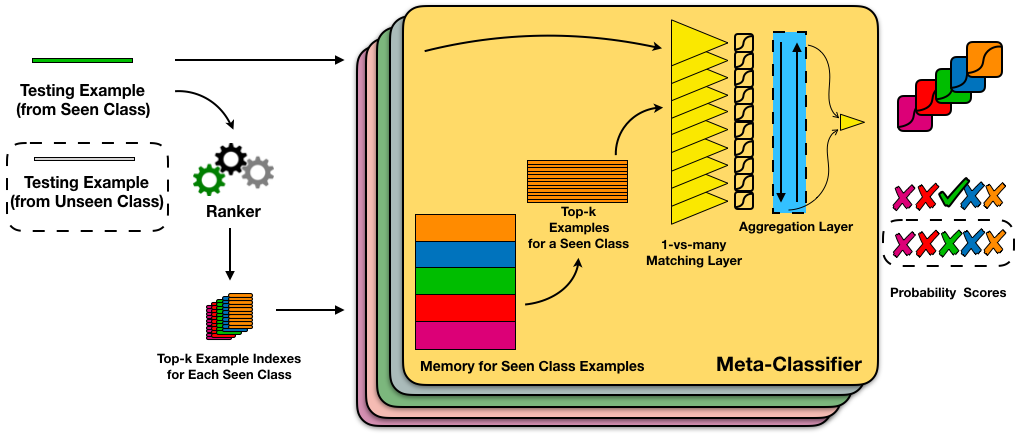
\includegraphics[width=5.7in]{fig/www19_overview.png}
%\caption{Overview of the L2AC framework (best viewed in colors). Assume the seen class set $S$ has 5 classes and their examples are indicated by 5 different colors. L2AC has two components: a ranker and a meta-classifier. Given a (green) testing example from a seen class, the ranker first retrieves the top-$k$ nearest examples (memory indexes) from each seen class. Then the meta-classifier takes both the test example and the top-$k$ nearest examples for a seen class to produce a probability score for that class. The meta-classifier is applied 5 times (indicated by 5 rounded rectangles) over these 5 seen classes and yields 5 probability scores, where the 3rd (green) class attends the maximum score as the final class (green) prediction. However, if the test example (grey) is from an unseen class (as indicated by the dashed box), none of those probability scores from the seen classes will predict positive, which leads rejection.}
\caption{Overview of the L2AC framework}
\label{chap2:fig:overview}
\end{figure*}

%\subsection{Meta-Classifier}
\textbf{Meta-Classifier}

Meta-classifier serves as the core component of the L2AC framework. It is essentially a binary classifier on a given seen class. It takes the top-$k$ nearest examples (to the test example $x_t$) of the seen class as the input and determines whether $x_t$ belongs to that seen class or not.
In this part, we first describe how to represent examples of a seen class. Then we describe how the meta-classifier processes these examples together with the test example into an overall probability score (via a voting mechanism) for deciding whether the test example should belong to any seen class (classification) or not (rejection). Along with that we also describe how a joint decision is made for open-world classification over a set of seen classes. Finally, we describe how to train the meta-classifier via another set of meta-training classes and their examples.

%\subsubsection{Example Representation and Memory}
\textbf{Example Representation and Memory}
\label{chap2:sec:mem}

Representation learning lives at the heart of neural networks. 
Following the success of using pre-trained weights from large-scale image datasets (such as ImageNet \cite{russakovsky2015imagenet}) as feature encoders, we assume there is an encoder that captures almost all features for text classification.

Given an example $x$ representing a text document (a sequence of tokens), we obtain its continuous representation (a vector) via an encoder $h=g(x)$, where the encoder $g(\cdot)$ is typically a neural network (e.g., CNN or LSTM).
We will detail a simple encoder implementation in Chapter \ref{chap2:sec:exp}.

Further, we save the continuous representations of the examples into the memory of the meta-classifier.
So later, the top-$k$ examples can be efficiently retrieved via the index (address) in the memory. 
The memory is essentially a matrix $E \in \mathbb{R} ^{n \times |h|}$, where $n$ means the total number of examples from seen classes and $|h|$ is the size of the hidden dimensions.
Note that we will still use $x$ instead of $h$ to refer to an example for brevity.
Given the test example $x_t$, the meta-classifier first looks up the actual continuous representations $x_{a_{1:k} }$ of the top-$k$ examples for a seen class.
Then the meta-classifier computes the similarity score between $x_t$ and each $x_{a_{i} }$ ($1\le i \le k$) individually via a 1-vs-many matching layer as described next. 

%\subsubsection{1-vs-many Matching Layer}
\textbf{1-vs-many Matching Layer}
\label{chap2:sec:1vsmany}

To compute the overall probability between a test example and a seen class, a 1-vs-many matching layer in the meta-classifier first computes the individual similarity score between the test example and each of the top-$k$ retrieved examples of the seen class. 
The 1-vs-many matching layer essentially consists of $k$ shared matching networks as indicated by big yellow triangles in \ref{chap2:fig:overview}.
We denote each matching network as $f(\cdot, \cdot)$ and compute similarity scores $r_{1:k}$ for all top-$k$ examples $r_{1:k}=f(x_t, x_{a_{1:k}} )$.

The matching network first transforms the test example $x_t$ and $x_{a_{i}}$ from the continuous representation space to a single example in similarity space.
We leverage two similarity functions to obtain the similarity space.
The first function is the absolute values of the element-wise subtraction:
$f_\text{abssub}(x_t, x_{a_{i}})=|x_t - x_{a_{i}}|$.
The second one is the element-wise summation:
$f_\text{sum}(x_t, x_{a_{i}})=x_t + x_{a_{i}}$.
Then the final similarity space is the concatenation of these two functions' results:
$f_\text{sim}(x_t, x_{a_{i}})=f_\text{abssub}(x_t, x_{a_{i}}) \oplus f_\text{sum}(x_t, x_{a_{i}})$, where $\oplus$ denotes the concatenation operation.
We then pass the result to two fully-connected layers (one with Relu activation) and a sigmoid function: 
\begin{equation}
\label{chap2:eq:r}
r_i=f(x_t, x_{a_i} )=\sigma\Big(W_2\cdot\text{Relu}\big(W_1\cdot f_\text{sim}(x_t, x_{a_i} ) +b_1\big)+b_2\Big).
\end{equation}
Since there are $k$ nearest examples, we have $k$ similarity scores denoted as $r_{1:k}$.
The hyper-parameters are detailed in Chapter \ref{chap2:sec:exp}.

%\subsubsection{Open-world Learning via Aggregation Layer}
\textbf{Open-world Learning via Aggregation Layer}
\label{chap2:sec:agg}

After getting the individual similarity scores, an aggregation layer in the meta-classifier merges the $k$ similarity scores into a single probability indicating whether the test example $x_t$ belongs to the seen class.
By having the aggregation layer, the meta-classifier essentially has a \textit{parametric voting mechanism} so that it can learn how to vote on multiple nearest examples (rather than a single example) from a seen class to decide the probability.
As a result, the meta-classifier can have more reliable predictions, which is studied in Chapter \ref{chap2:sec:exp}.

We adopt a (many-to-one) BiLSTM \cite{hochreiter1997long,schuster1997bidirectional} as the aggregation layer.
We set the output size of BiLSTM to 2 (1 per the direction of LSTM). 
Later, the output hidden states of BiLSTM are connected to a dense layer followed by a sigmoid function that outputs the probability.
The computation of the meta-classifier for a given test example $x_t$ and $x_{a_{1:k}}$ for a seen class $c$ can be summarized as: 
\begin{equation}
    \label{chap2:eq:p}
p(c|x_t, x_{a_{1:k}} )=\sigma\big(W\cdot \text{BiLSTM}(r_{1:k})+b\big).
\end{equation}
%Lastly,
Inspired by DOC \cite{shu-xu-liu:2017:EMNLP2017}, 
for each class $c \in S$, we evaluate \ref{chap2:eq:p} as:
\begin{equation} 
    \label{chap2:eq:rej}
        \hat{y} = \left\{
        \begin{array}{c}
        \textit{reject}, \text{ if } \max_{c \in S} p(c|x_t, x_{a_{1:k}} ) \le 0.5 ;\\
        \\
        \argmax_{c \in S} p(c|x_t, x_{a_{1:k}} ) ,\text{ otherwise.}
        \end{array} \right.
    %     }
\end{equation}
If none of existing seen classes $S$ gives a probability above $0.5$, we \emph{reject} $x_t$ as an example from some unseen class.
Note that given a large number of classes, \ref{chap2:eq:rej} can be efficiently implemented in parallel. We leave this to future work.
To make L2AC an easily accessible approach, we use $0.5$ as the threshold naturally and do not introduce an extra hyper-parameter that needs to be artificially tuned.
Note also that as discussed earlier, the seen class set $S$ and its examples can be dynamically maintained (e.g., one can add to or remove from $S$ any class). So the meta-classifier simply performs open-world classification over the current seen class set $S$.

\textbf{Training of Meta-Classifier}
\label{chap2:sec:train}

Since the meta-classifier is a general classifier that is supposed to work for any class,
training the meta-classifier $p_\theta(c|x_t, x_{a_{1:k}|x_t, c} )$
requires examples from another set $M$ of classes called \textit{meta-training classes}.

A large $|M|$ is desirable so that meta-training classes have good coverage of features for seen and unseen classes in testing, which is in a similar spirit to few-shot learning \cite{lake2011one}. 
We also enforce $ (S\cup U) \cap M=\varnothing$ in Chapter \ref{chap2:sec:exp}, so that all seen and unseen classes are unknown to the meta-classifier.

Next, we formulate the meta-training examples from $M$, which consist of a set of pairs 
(with positive and negative labels). 
The first component of a pair is a training document $x_q$ from a class in $M$, and the second component is a sequence of top-$k$ nearest examples also from a class in $M$. 

We assume every example (document) of a class in $M$ can be a training document $x_q$.
Assuming $x_q$ is from class $c \in M$,
a positive training pair is $(x_q, x_{a_{1:k}|x_q, c})$, where $x_{a_{1:k}|x_q, c}$ are top-$k$ examples from class $c$ that are most similar or nearest to $x_q$;
a negative training pair is $(x_q, x_{a_{1:k}|x_q, c'})$, where $c' \in M$, $c \neq c'$ and $x_{a_{1:k}|x_q, c'}$ are top-$k$ examples from class $c'$ that are nearest to $x_q$.
We call $c'$ one \emph{negative class} for $x_q$.
Since there are many negative classes $c' \in M\backslash c$ for $x_q$, we keep top-$n$ negative classes for each training example $x_q$. 
That is, each $x_q$ has one positive training pair and $n$ negative training pairs.
To balance the classes in the training loss, we give a weight ratio $n:1$ for a positive and a negative pair, respectively.

Training the meta-classifier also requires validation classes for model selection (during optimization) and hyper-parameters ($k$ and $n$) tuning (as detailed in Experiments).
Since the classes tested by the meta-classifier are unexpected, we further use a set of  \textit{validation classes} $M'\cap M=\varnothing$ (also $M'\cap (S\cup U)=\varnothing$), to ensure generalization on the seen/unseen classes.

\section{Results}
\label{chap2:sec:exp}

We want to address the following Research Questions (RQs) in experiments:
\textbf{RQ1} - what is the performance of the meta-classifier with different settings of top-$k$ examples and $n$ negative classes?
\textbf{RQ2} - How is the performance of L2AC compared with state-of-the-art text classifiers for open-world classification (which all need some forms of re-training).

%\subsection{Dataset}
\textbf{Dataset}

We leverage the huge amount of product descriptions from the Amazon Datasets \cite{he2016ups} and form the OWL task as the following.
Amazon.com maintains a tree-structured category system. 
We consider each path to a leaf node as a class.
We removed products belonging to multiple classes to ensure the classes have no overlapping.
This gives us 2598 classes, where 1018 classes have more than 400 products per class.
We randomly choose 1000 classes from the 1018 classes with 400 randomly selected products per class as the \textit{encoder training set};
100 classes with 150 products per class are used as the (classification) \textit{test set}, including both seen classes $S$ and unseen classes $U$;
another 1000 classes with 100 products per class are used as the \textit{meta-training set} (including both $M$ and $M'$).
For the 100 classes of the test set, we further hold out 50 examples (products) from each class as test examples. 
The rest 100 examples are training data for baselines, or seen classes examples to be read by the meta-classifier (which only reads those examples but is not trained on those examples).
To train the meta-classifier, we further split the meta-training set as 900 \textit{meta-training classes} ($M$) and 100 \textit{validation classes} ($M'$).
For all datasets, we use NLTK(\url{https://www.nltk.org/}) as the tokenizer, and regard all words that appear more than once as the vocabulary.
This gives us 17,526 unique words.
We take the maximum length of each document as 120 since the majority of product descriptions are under 100 words.

\textbf{Ranker}

We use cosine similarity to rank the examples in each seen (or meta-training) class for a given test (or meta-training) example $x_t$ (or $x_q$)(Given many examples to process, the ranker can be implemented in a fully parallel fashion to speed up the processing, which we leave to future work as it is beyond the scope of this work.).
We apply cosine directly on the hidden representations of the encoder as $cosine(h_*, h_{a_{i}})=\frac{h_* \cdot h_{a_{i}}}{|h_*|_2|h_{a_{i}}|_2}$, where $*$ can be either $t$ or $q$, $|\cdot|_2$ denotes the $l$-2 norm and $\cdot$ denotes the dot product of two examples.

Training the meta-classifier also requires a ranking of negative classes for a meta-training example $x_q$, as discussed in Chapter \ref{chap2:sec:train}.
We first compute a \textit{class vector} for each meta-training class. 
This class vector is averaged over all encoded representations of examples of that class.
Then we rank classes by computing cosine similarity between the class vectors and the meta-training example $x_q$.
The top-$n$ (defined in the previous section) classes are selected as negative classes for $x_q$.
We explore different settings of $n$ later.

\textbf{Evaluation}

Similar to \cite{shu-xu-liu:2017:EMNLP2017}, we choose 25, 50, and 75 classes from the (classification) test set of 100 classes as the seen classes for three (3) experiments.
Note that each class in the test set has 150 examples, where 100 examples are for the training of baseline methods or used as seen class examples for L2AC and 50 examples are for testing both the baselines and L2AC.
We evaluate the results on all 100 classes for those three (3) experiments.
For example, when there are 25 seen classes, testing examples from the rest 75 unseen classes are taken as from one \textit{rejection class} $c_\text{rej}$, as in \cite{shu-xu-liu:2017:EMNLP2017}.

Besides using macro F1 as used in \cite{shu-xu-liu:2017:EMNLP2017}, we also use weighted F1 score overall classes (including seen and the rejection class) as the evaluation metric.
Weighted F1 is computed as 
\begin{equation}
\sum_{c\in S\cup\{c_\text{rej}\} } \frac{N_c}{\sum_{c\in S\cup\{c_\text{rej}\}}N_c  }\cdot \text{F1}_c,
\end{equation}
where $N_c$ is the total number of examples for class $c$. $\text{F1}_c$ is the F1 score of that class.
We use this metric because macro F1 has a bias on the importance of rejection when the seen class set is small (macro F1 treats the rejection class as equally important as one seen class).
For example, when the number of seen classes is small, the rejection class should have a higher weight as a classifier on a small seen set is more likely challenged by examples from unseen classes.
Further, to stabilize the results, we train all models with 10 different initializations and average the results.

\textbf{Hyper-parameters}

For simplicity, we leverage a BiLSTM \cite{hochreiter1997long,schuster1997bidirectional} on top of a GloVe \cite{pennington2014glove} embedding (840b.300d) layer as the encoder (other choices are also possible).
Similar to feature encoders trained from ImageNet~\cite{russakovsky2015imagenet}, we train classification over the encoder training set with 1000 classes and use 5\% of the encoding training data as encoder validation data.
We apply dropout rates of 0.5 to all layers of the encoder. 
The classification accuracy of the encoder on validation data is \textbf{81.76\%}.
The matching network (the shared network within the 1-vs-many matching layer) has two fully-connected layers, where the size of the hidden dimension is 512 with a dropout rate of 0.5.
We set the batch size of meta-training as 256.

To answer RQ1 on two hyper-parameters $k$ (number of nearest examples from each class) and $n$ (number of negative classes), we use the 100 validation classes to determine these two hyper-parameters.
We formulate the validation data similar to the testing experiment on 50 seen classes.
For validation, we select 50 examples for each class. The rest 50 examples from each validation seen class are used to find top-$k$ nearest examples.
We perform grid search of averaged weighted F1 over 10 runs for $k\in\{1, 3, 5, 10, 15, 20\}$ and $n\in \{1, 3, 5, 9\}$, where \textbf{$k=5$} and \textbf{$n=9$} reach a reasonably well weighted F1 (87.60\%). Further increasing $n$ gives limited improvements (e.g., 87.69\% for $n=14$ and 87.68\% for $n=19$, when $k=5$). But a large $n$ significantly increases the number of training examples (e.g., $n=14$ ended with more than 1 million meta-training examples) and thus training time. So we decide to select $k=5$ and $n=9$ for all ablation studies below.
Note the validation classes are also used to compute (formulated in a way similar to the meta-training classes) the validation loss for selecting the best model during Adam \cite{kingma2014adam} optimization.

\textbf{Compared Methods}

\begin{table*}[t]
\centering    
\scalebox{0.7}{

\begin{tabular}{l||c|c|c|c|c|c}
\hline
{\bf Methods} & $|S|=25$ (WF1) & $|S|=25$ (MF1) & $|S|=50$ (WF1) & $|S|=50$ (MF1) & $|S|=75$ (WF1) & $|S|=75$ (MF1) \\
\hline
DOC-CNN & 53.25(1.0) & 55.04(0.39) & 70.57(0.46) & 76.91(0.27) & 81.16(0.47) & 86.96(0.2) \\
DOC-LSTM & 57.87(1.26) & 57.6(1.18) & 69.49(1.58) & 75.68(0.78) & 77.74(0.48) & 84.48(0.33) \\
DOC-Enc & 82.92(0.37) & 75.09(0.33) & 82.53(0.25) & 84.34(0.23) & 83.84(0.36) & 88.33(0.19) \\
\hline
DOC-CNN-Gaus & 85.72(0.43) & 76.79(0.41) & 83.33(0.31) & 83.75(0.26) & 84.21(0.12) & 87.86(0.21) \\
DOC-LSTM-Gaus & 80.31(1.73) & 70.49(1.55) & 77.49(0.74) & 79.45(0.59) & 80.65(0.51) & 85.46(0.25) \\
DOC-Enc-Gaus & 88.54(0.22) & 80.77(0.22) & 84.75(0.21) & 85.26(0.2) & 83.85(0.37) & 87.92(0.22) \\
\hline
\hline
L2AC-$n$9-NoVote & 91.1(0.17) & 82.51(0.39) & 84.91(0.16) & 83.71(0.29) & 81.41(0.54) & 85.03(0.62) \\
L2AC-$n$9-Vote3 & 91.54(0.55) & 82.42(1.29) & 84.57(0.61) & 82.7(0.95) & 80.18(1.03) & 83.52(1.14) \\
\hline
L2AC-$k$5-$n$9-AbsSub & 92.37(0.28) & 84.8(0.54) & 85.61(0.36) & 84.54(0.42) & 83.18(0.38) & 86.38(0.36) \\
L2AC-$k$5-$n$9-Sum & 83.95(0.52) & 70.85(0.91) & 76.09(0.36) & 75.25(0.42) & 74.12(0.51) & 78.75(0.57) \\
\hline
L2AC-$k$\textbf{5}-$n$\textbf{9} & \underline{93.07}(0.33) & 86.48(0.54) & \underline{86.5}(0.46) & 85.99(0.33) & \underline{84.68}(0.27) & 88.05(0.18) \\
L2AC-$k$5-$n$14 & \textbf{93.19}(0.19) & 86.91(0.33) & \textbf{86.63}(0.28) & 86.42(0.2) & 85.32(0.35) & 88.72(0.23) \\
L2AC-$k$5-$n$19 & 93.15(0.24) & 86.9(0.45) & 86.62(0.49) & 86.48(0.43) & \textbf{85.36}(0.66) & 88.79(0.52) \\
\hline
\end{tabular}
    }
\caption{Scores for OWL}

 \vspace{-3mm}
\label{chap2:tbl:result}
\end{table*}

%\caption{Weighted F1 (WF1) and macro F1 (MF1) scores on a test set with 100 classes with 3 settings: 25, 50, and 75 seen classes. The set of seen classes is incrementally expanded from 25 to 75 classes (or gradually shrunk from 75 to 25 classes). The results are the averages over 10 runs with standard deviations in parenthesis.}

\begin{figure*}
\center
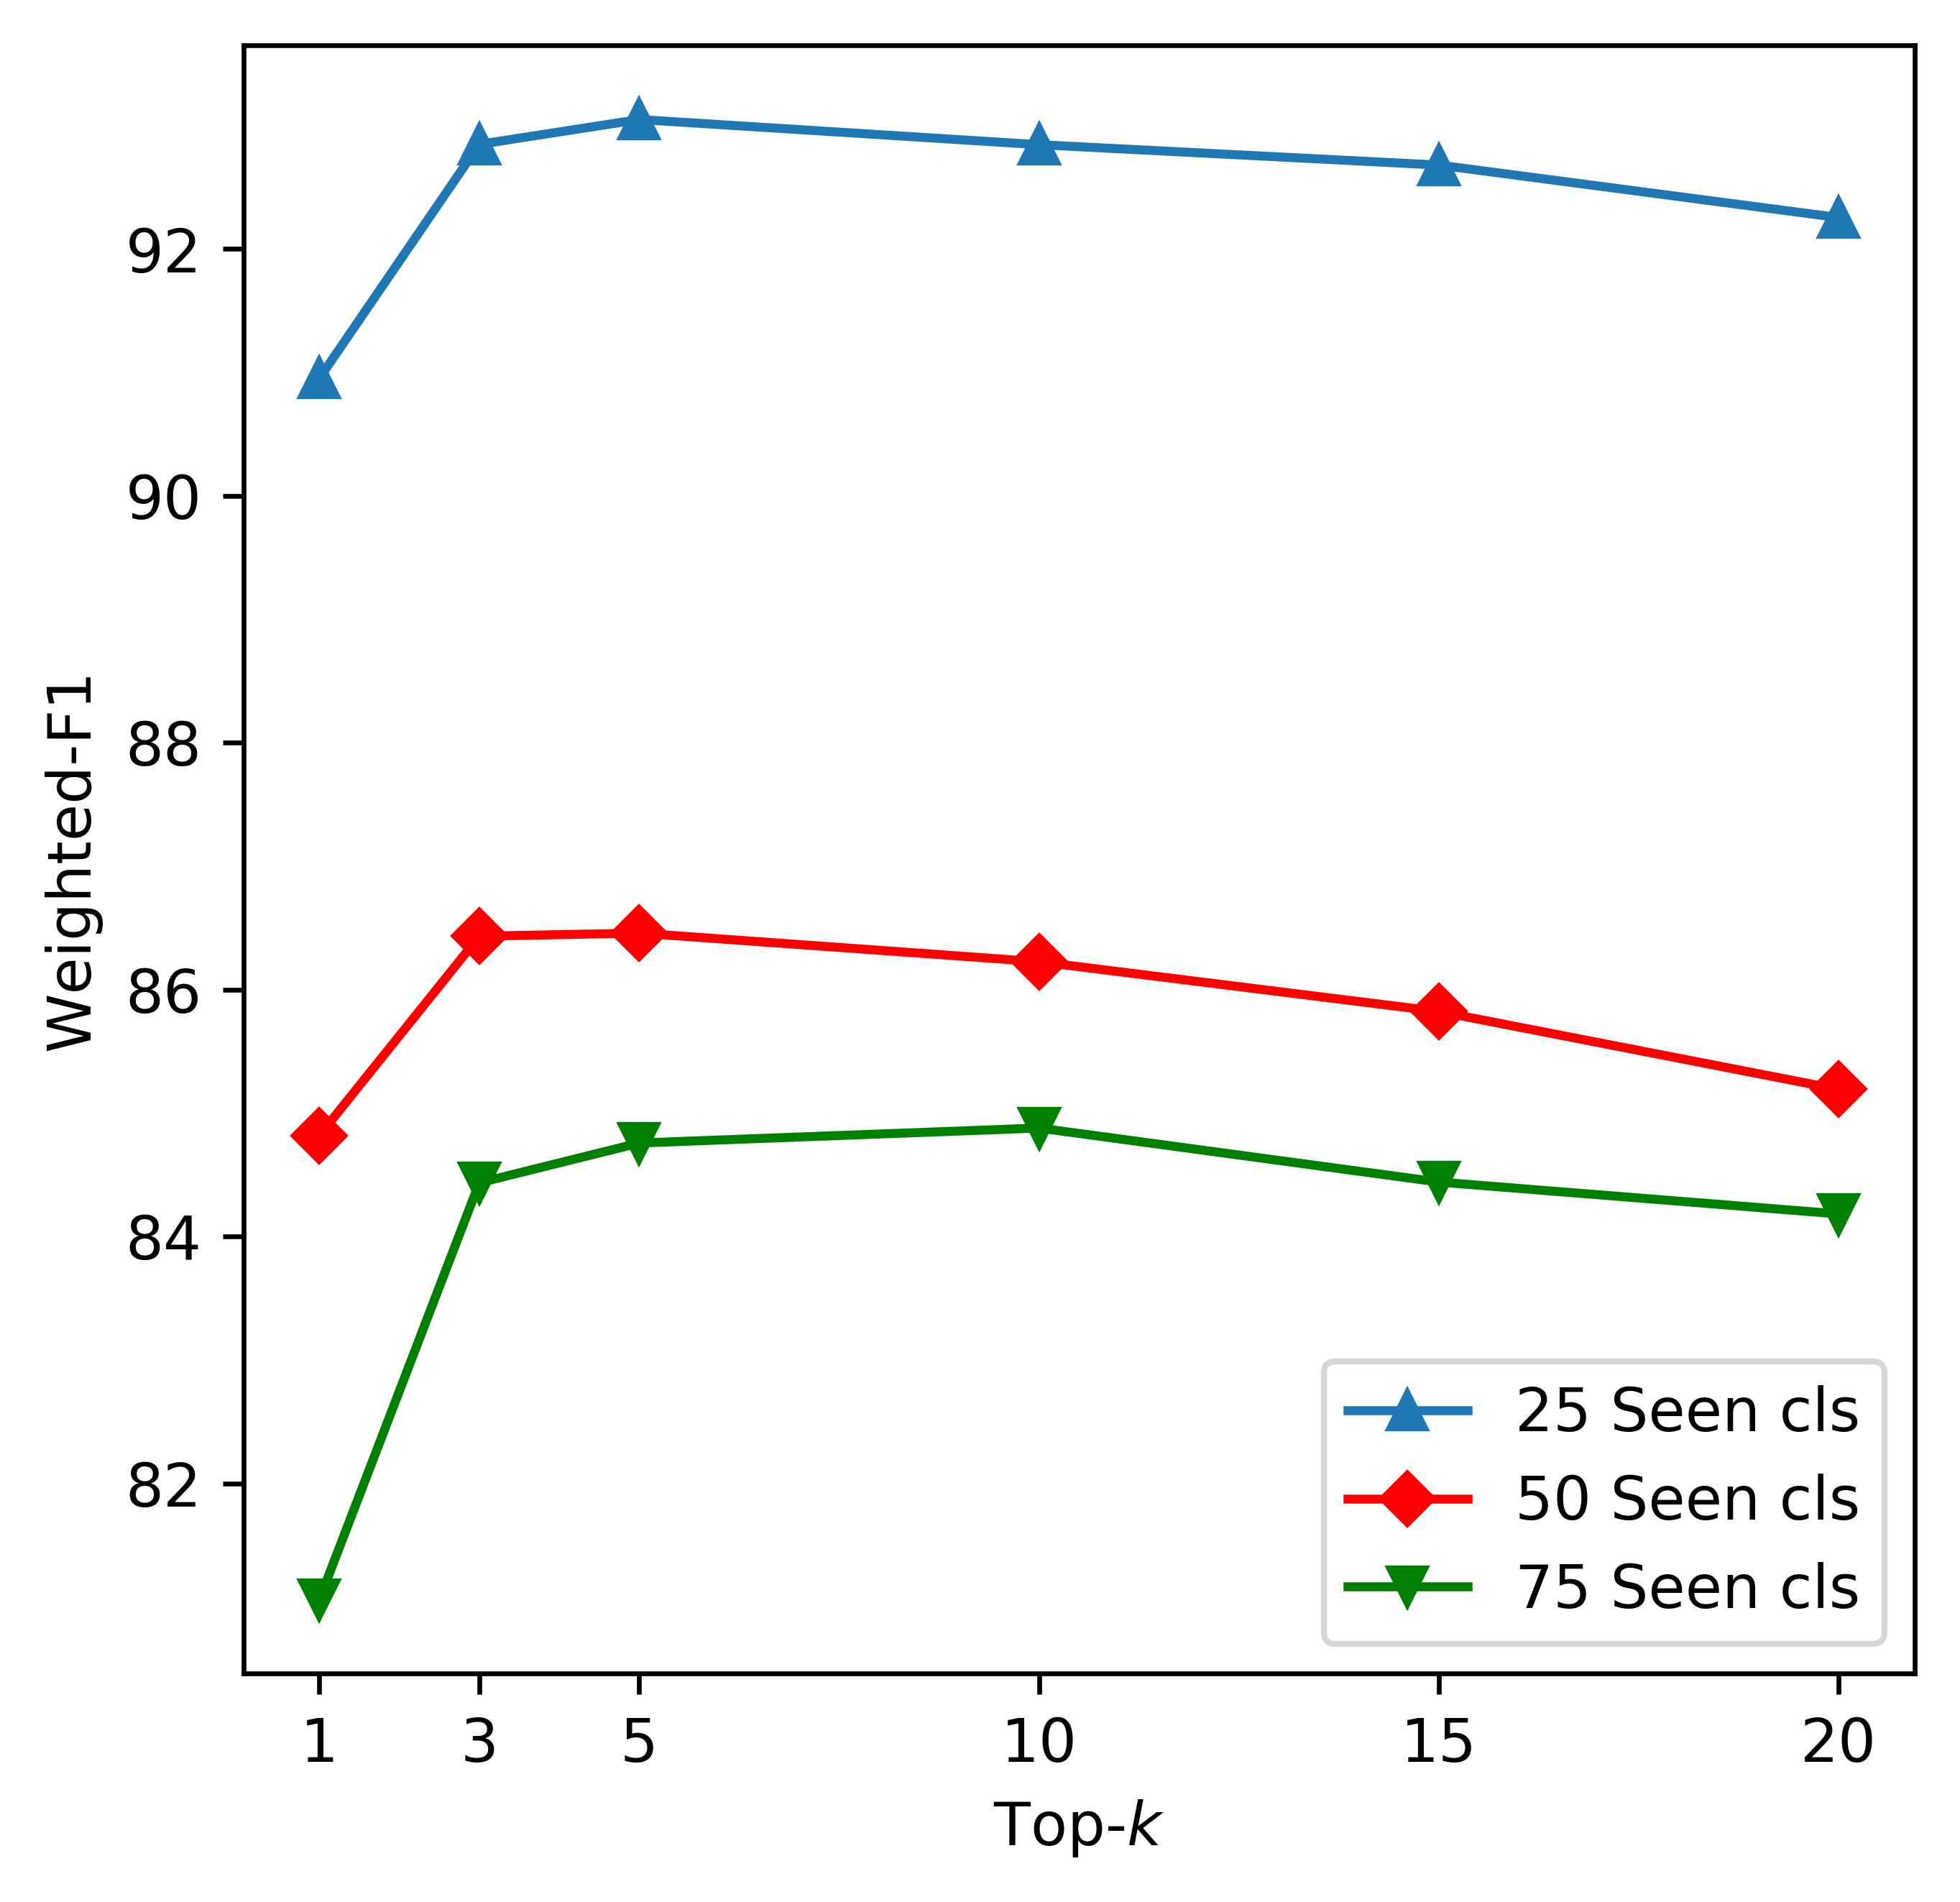
\includegraphics[width=2.5in]{fig/www19_top_k.png}
\quad
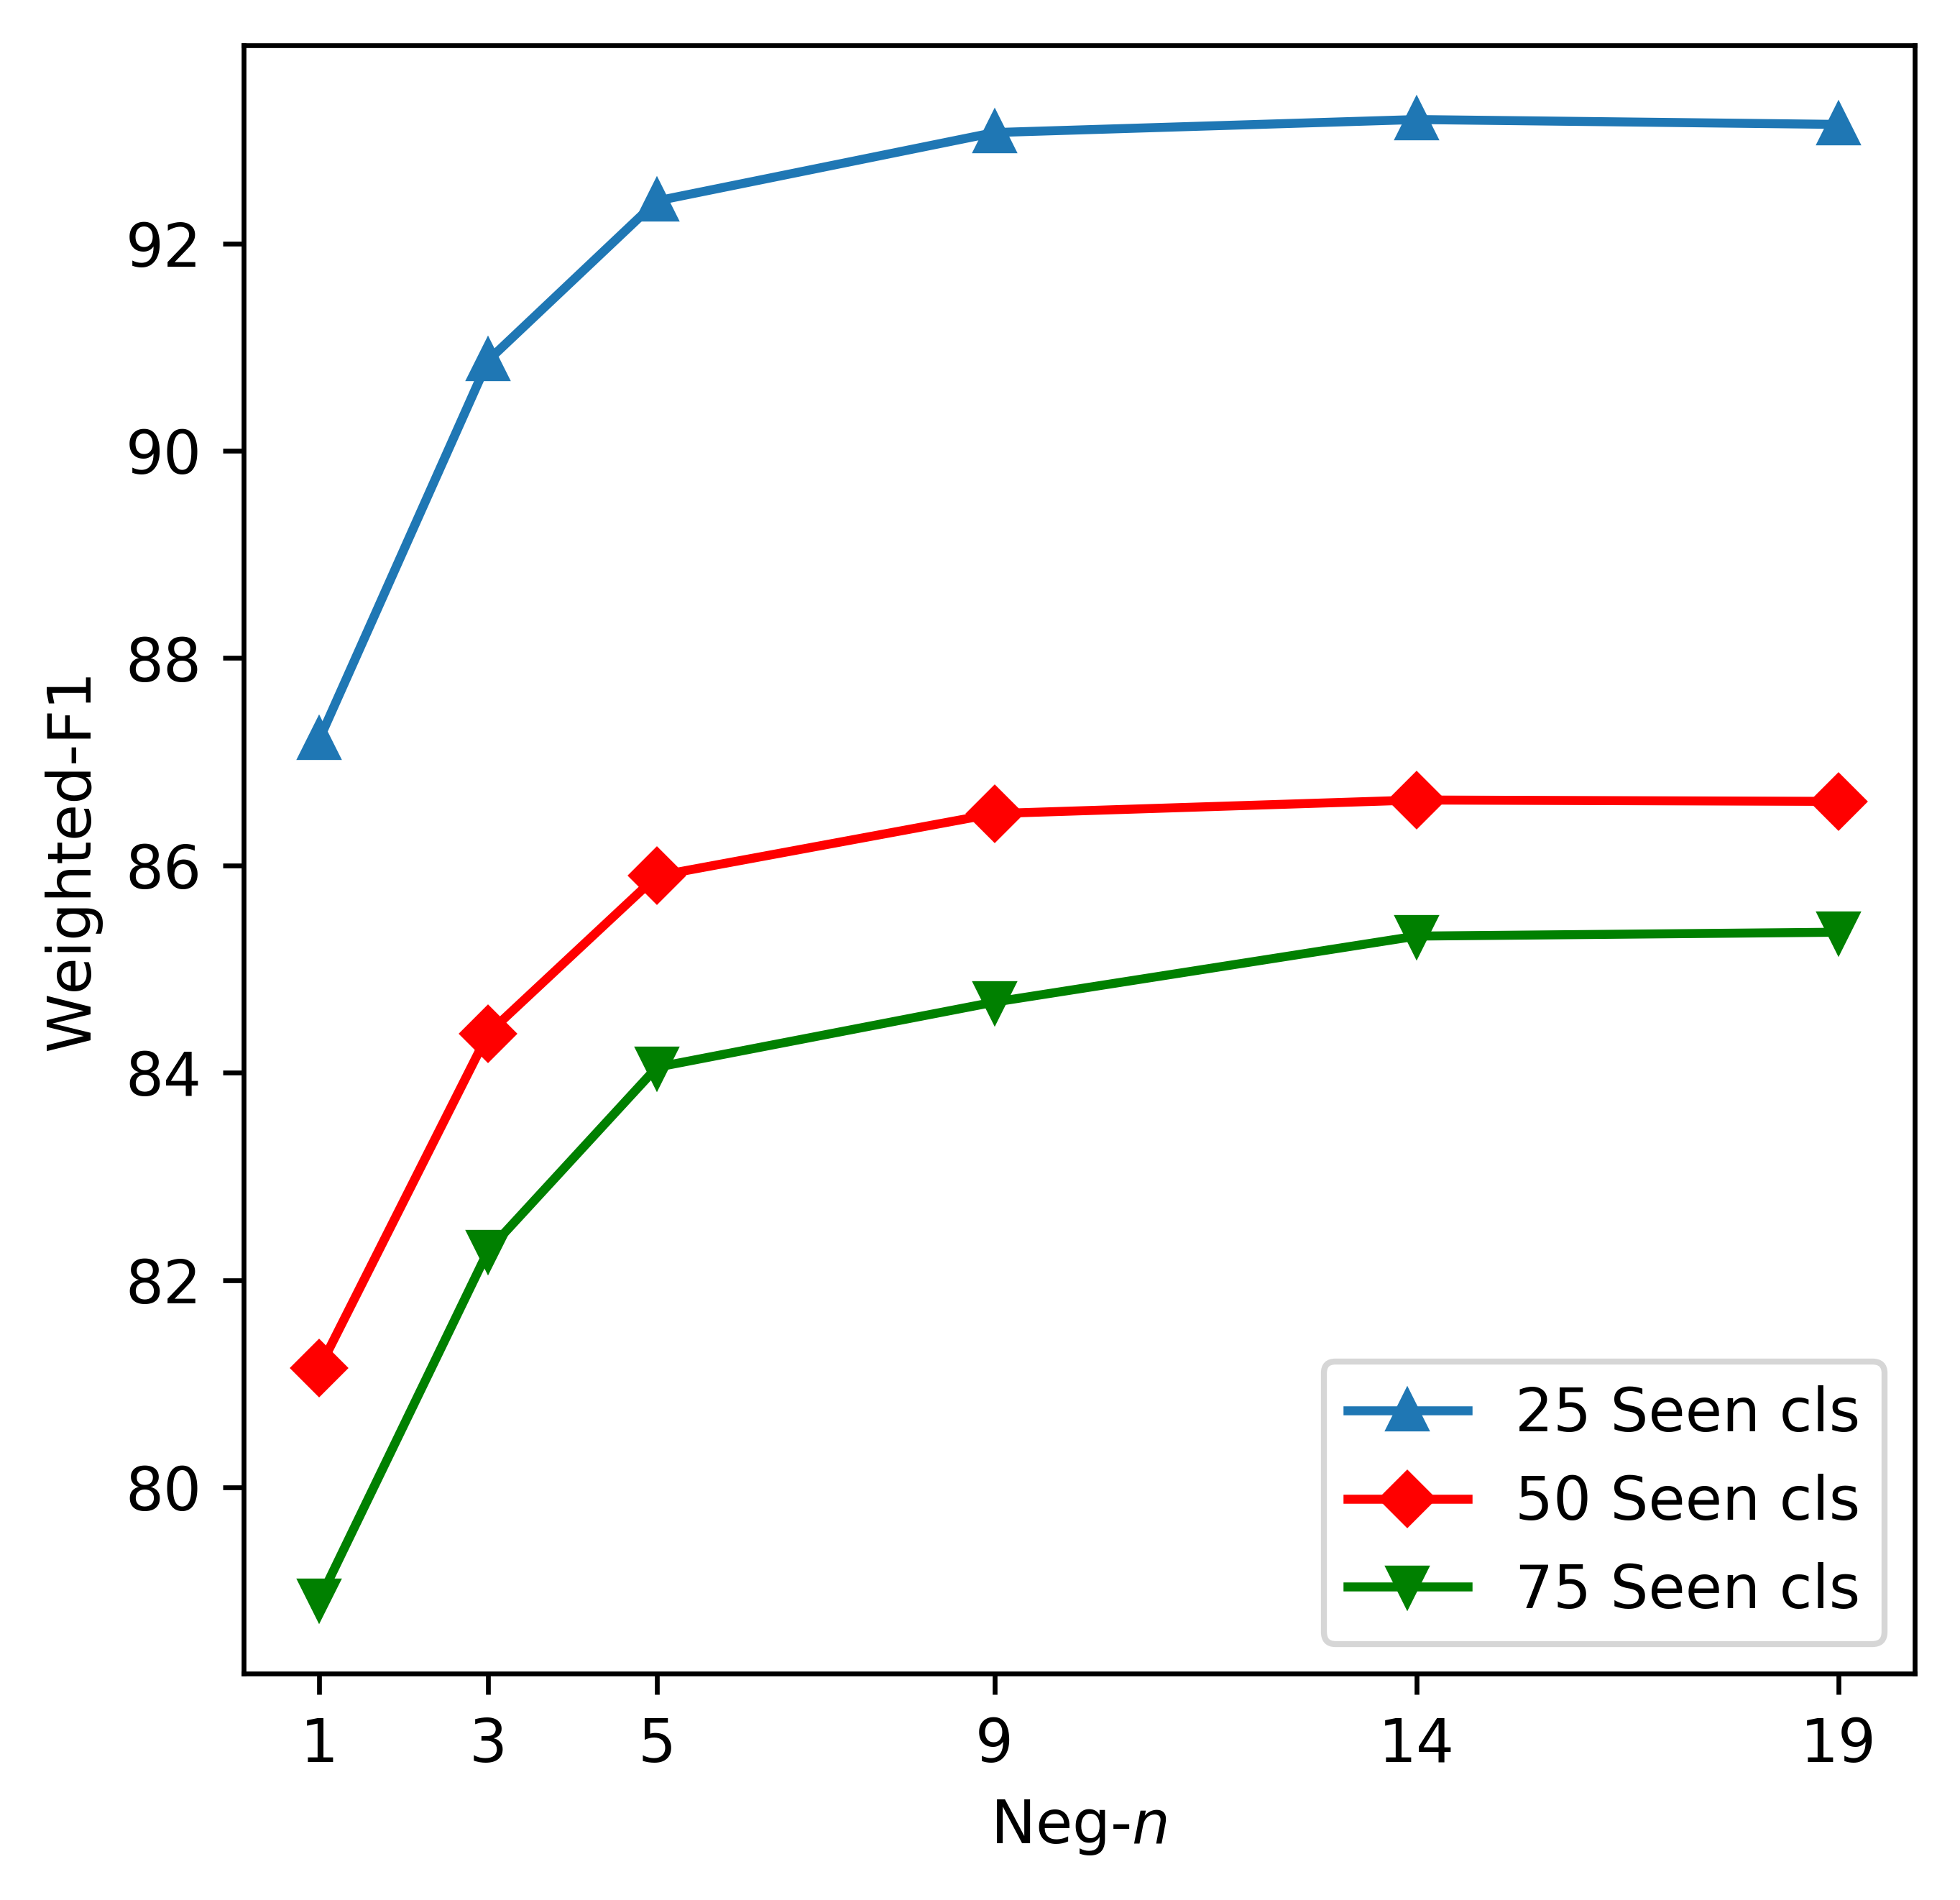
\includegraphics[width=2.5in]{fig/www19_neg_n.png}
%\caption{Weighted F1 scores for different $k$'s ($n=9$) and different $n$'s ($k=5$).}
\caption{Weighted F1 scores of $k$ and $n$ for OWL}
\label{chap2:fig:kn}
\end{figure*}

DOC \cite{shu-xu-liu:2017:EMNLP2017} is a state-of-the-art baseline for text classification in the open-world learning (with rejection) setting. It has been shown in \cite{shu-xu-liu:2017:EMNLP2017} that DOC significantly outperforms the methods CL-cbsSVM and cbsSVM in~\cite{fei2016learning} and OpenMax in~\cite{bendale2016towards}. OpenMax is a state-of-the-art method for image classification with rejection capability. 
To answer RQ2, we use DOC and its variants to show that the proposed method has comparable performance with the best open-world learning method with re-training.
Note that DOC cannot incrementally add new classes. 
So we re-train DOC over different sets of seen classes from scratch every time new classes are added to that set.

It is thus actually unfair to compare our method with DOC because DOC is trained on the actual training examples of all classes. However, our method still performs better in general. We used the original code of DOC and created six (6) variants of it.

\vspace{+2mm}
\noindent
\textbf{DOC-CNN}: CNN implementation as in the original DOC paper without Gaussian fitting (using 0.5 as the threshold for rejection). It operates directly on a sequence of tokens. \\
\textbf{DOC-LSTM}: a variant of DOC-CNN, where we replace CNN with BiLSTM to encode the input sequence for a fair comparison. BiLSTM is trainable and the input is still a sequence of tokens. \\
\textbf{DOC-Enc}: this is adapted from DOC-CNN, where we remove the feature learning part of DOC-CNN and feed the hidden representation from our encoder directly to the fully-connected layers of DOC for a fair comparison with L2AC. \\
\textbf{DOC-*-Gaus}: applying Gaussian fitting proposed in \cite{shu-xu-liu:2017:EMNLP2017} on the above three baselines, we have 3 more DOC baselines. 
Note that these 3 baselines have the same models as above respectively. They only differ in the thresholds used for rejection. Gaussian fitting in \cite{shu-xu-liu:2017:EMNLP2017} is used to set a good threshold for rejection. 
We use these baselines to show that the Gaussian fitted threshold improves the rejection performance of DOC significantly but may lower the performance of seen class classification. The original DOC is \textbf{DOC-CNN-Gaus} here. 

\vspace{+1mm}
The following baselines are variants of L2AC.\\
\textbf{L2AC-$n$9-NoVote}: this is a variant of the proposed L2AC that only takes one most similar example (from each class), i.e., $k=1$, with one positive class paired with $n=9$ negative classes in meta-training ($n=9$ has the best performance as indicated in answering RQ1 above). 
We use this baseline to show that the performance of taking only one sample may not be good enough.
This baseline does not have/need the aggregation layer and only has a single matching network in the 1-vs-many layer.\\
\textbf{L2AC-$n$9-Vote3}: this baseline uses the same model as L2AC-$n$9-NoVote. But during the evaluation, we allow a non-parametric voting process (like $k$NN) for prediction. We report the results of voting over top-3 examples per seen class as it has the best result (ranging from 3 to 10). If the average of the top-3 similar examples in a seen class has example scores with more than $0.5$, L2AC believes the testing example belongs to that class.
We use this baseline to show that the aggregation layer is effective in learning to vote and L2AC can use more similar examples and get better performance.\\

\textbf{L2AC-$k$5-$n$9-AbsSub/Sum}: To show that using two similarity functions ($f_\text{abssub}(\cdot, \cdot)$ and $f_\text{sum}(\cdot, \cdot)$ ) gives better results, we further perform ablation study by using only one of those similarity functions at a time, which gives us two baselines.\\
\textbf{L2AC-$k$5-$n$9/14/19}: this baseline has the best $k=5$ and $n=9$ on the validation classes, as indicated in the previous subsection. Interestingly, further increasing $k$ may reduce the performance as L2AC may focus on not-so-similar examples. We also report results on $n=14$ or $19$ to show that the results do not get much better. 

\textbf{Results Analysis}

From Table \ref{chap2:tbl:result}, we can see that L2AC outperforms DOC, especially when the number of seen classes is small. 
First, from \ref{chap2:fig:kn} we can see that $k=5$ and $n=9$ gets reasonably good results.
Increasing $k$ may harm the performance as taking in more examples from a class may let L2AC focus on not-so-similar examples, which is bad for classification. More negative classes give L2AC better performance in general but further increasing $n$ beyond 9 has little impact.

Next, we can see that as we incrementally add more classes, L2AC gradually drops its performance (which is reasonable due to more classes) but it still yields better performance than DOC. Considering that L2AC needs no training with additional classes, while DOC needs full training from scratch, L2AC  represents a major advance. Note that testing on 25 seen classes is more about testing a model's rejection capability while testing on 75 seen classes is more about the classification performance of seen class examples.
From \ref{chap2:tbl:result}, we notice that L2AC can effectively leverage multiple nearest examples and negative classes.
In contrast, the non-parametric voting of L2AC-$n$9-Vote3 over top-3 examples may not improve the performance but introduce higher variances.
Our best $k=5$ indicates that the meta-classifier can dynamically leverage multiple nearest examples instead of solely relying on a single example.
As an ablation study on the choices of similarity functions, running L2AC on a single similarity function gives poorer results as indicated by either L2AC-$k$5-$n$9-AbsSub or L2AC-$k$5-$n$9-Sum.

DOC without encoder (DOC-CNN or DOC-LSTM) performs poorly when the number of seen classes is small.
Without Gaussian fitting, DOC's (DOC-CNN, DOC-LSTM or DOC-Enc) performance increases as more classes are added as seen classes. This is reasonable as DOC is more challenged by fewer seen training classes and more unseen classes during testing. 
As such, Gaussian fitting (DOC-*-Gaus) alleviates the weakness of DOC on a small number of seen training classes.

